\documentclass[aspectratio=169]{beamer}

% Shared Beamer settings for Applied Machine Learning lectures (UPES).
% Keep this file free of \documentclass to allow reuse via \input.

% Allow lecture sources to use shared theme/assets without copying them into each lecture folder.
% NOTE: These paths are relative to `Unit-xx/Lecture-yy/latex/` (and `Lab/Experiment-xx/latex/`).
\makeatletter
\def\input@path{{../../../_shared/}{../../../_shared/UPES-Beamer-Theme/}}
\makeatother

\usetheme{UPES}
\setbeamertemplate{navigation symbols}{}

\usepackage{amsmath}
\usepackage{amssymb}
\usepackage{booktabs}
\usepackage{graphicx}
\usepackage{hyperref}
\usepackage{xcolor}
\usepackage{listings}

% Code listings (Python-oriented for this subject).
\lstset{
  language=Python,
  basicstyle=\ttfamily\small,
  keywordstyle=\color{blue},
  commentstyle=\color{gray},
  stringstyle=\color{teal},
  showstringspaces=false,
  columns=fullflexible,
  breaklines=true
}

\usepackage{tikz}
\usetikzlibrary{arrows.meta,positioning,shapes.geometric,calc,fit,backgrounds}

% Per-slide source line (references shown on the slide itself).
\newcommand{\slidesources}[1]{%
  \vfill
  {\tiny\color{gray}\raggedright\sloppy\parbox{\linewidth}{Sources: #1}\par}%
}

% Unit-wise source strings for this subject (used by slides/notes).
% Path is relative to the lecture `latex/` folder (the compilation CWD).
% Source strings for Applied Machine Learning (CSAI2017P) — used by slides + notes.
% Prescribed texts and reference books are taken from the course syllabus.
% Support texts are the author-hosted open-access editions:
%   statlearning.com            (ISL with Python)
%   probml.github.io/pml-book   (Murphy, Probabilistic Machine Learning)
%   d2l.ai                      (Dive into Deep Learning)
%   mml-book.github.io          (Mathematics for Machine Learning)

\newcommand{\AMLRepoURL}{https://github.com/tali7c/Applied-Machine-Learning}

% --- prescribed -------------------------------------------------------------
\newcommand{\AMLPrescribed}{%
M\"uller and Guido, \textit{Introduction to Machine Learning with Python}, O'Reilly, 2016.;%
Bishop, \textit{Pattern Recognition and Machine Learning}, Springer, 2006.;%
Murphy, \textit{Machine Learning: A Probabilistic Perspective}, MIT Press, 2012.;%
Han, Kamber and Pei, \textit{Data Mining: Concepts and Techniques} (3e), Morgan Kaufmann, 2012.%
}

% --- unit-wise ---------------------------------------------------------------
\newcommand{\AMLUnitISources}{%
M\"uller and Guido, \textit{Introduction to Machine Learning with Python}, Ch. 1.;%
Bishop, \textit{Pattern Recognition and Machine Learning}, Ch. 1.;%
Murphy, \textit{Probabilistic Machine Learning: An Introduction}, MIT Press, 2022, Ch. 1.;%
Mitchell, \textit{Machine Learning}, McGraw Hill, 1997, Ch. 1.;%
Scikit-learn documentation, accessed 2026-08-04.%
}

\newcommand{\AMLUnitIISources}{%
Bishop, \textit{Pattern Recognition and Machine Learning}, \S1.5, \S4.3, \S7.1.;%
Zhang, Lipton, Li and Smola, \textit{Dive into Deep Learning}, \S3.4.;%
Shalev-Shwartz and Ben-David, \textit{Understanding Machine Learning}, Ch. 15.;%
Murphy, \textit{Probabilistic Machine Learning: An Introduction}, Ch. 5.%
}

\newcommand{\AMLUnitIIISources}{%
Zhang, Lipton, Li and Smola, \textit{Dive into Deep Learning}, Ch. 12 (Optimization Algorithms).;%
Deisenroth, Faisal and Ong, \textit{Mathematics for Machine Learning}, Ch. 7.;%
Kingma and Ba, ``Adam: A Method for Stochastic Optimization,'' ICLR 2015.;%
Ruder, ``An overview of gradient descent optimization algorithms,'' arXiv:1609.04747, 2016.%
}

\newcommand{\AMLUnitIVSources}{%
Han, Kamber and Pei, \textit{Data Mining: Concepts and Techniques} (3e), Ch. 3.;%
M\"uller and Guido, \textit{Introduction to Machine Learning with Python}, Ch. 3--4.;%
James, Witten, Hastie, Tibshirani and Taylor, \textit{An Introduction to Statistical Learning with Python}, Ch. 5--6, 12.;%
Scikit-learn documentation (preprocessing, model selection), accessed 2026-08-04.%
}

\newcommand{\AMLUnitVSources}{%
James et al., \textit{An Introduction to Statistical Learning with Python}, Ch. 3--6.;%
Bishop, \textit{Pattern Recognition and Machine Learning}, Ch. 3.;%
Deisenroth, Faisal and Ong, \textit{Mathematics for Machine Learning}, Ch. 9.;%
M\"uller and Guido, \textit{Introduction to Machine Learning with Python}, \S2.3.%
}

\newcommand{\AMLUnitVISources}{%
Han, Kamber and Pei, \textit{Data Mining: Concepts and Techniques} (3e), Ch. 8--9.;%
James et al., \textit{An Introduction to Statistical Learning with Python}, Ch. 8--9.;%
Bishop, \textit{Pattern Recognition and Machine Learning}, Ch. 4--5, 7, 14.;%
Zhang et al., \textit{Dive into Deep Learning}, Ch. 5.%
}

\newcommand{\AMLUnitVIISources}{%
Han, Kamber and Pei, \textit{Data Mining: Concepts and Techniques} (3e), Ch. 10.;%
James et al., \textit{An Introduction to Statistical Learning with Python}, Ch. 12.;%
M\"uller and Guido, \textit{Introduction to Machine Learning with Python}, \S3.5.;%
Ester, Kriegel, Sander and Xu, ``A density-based algorithm for discovering clusters (DBSCAN),'' KDD 1996.%
}

\newcommand{\AMLLabSources}{%
M\"uller and Guido, \textit{Introduction to Machine Learning with Python}, companion notebooks.;%
McKinney, \textit{Python for Data Analysis} (3e), O'Reilly, 2022.;%
Scikit-learn user guide, accessed 2026-08-04.;%
Matplotlib and Seaborn documentation, accessed 2026-08-04.%
}



\graphicspath{{../figures/}{../images/}{../../../_shared/}{../../../_shared/UPES-Beamer-Theme/}}

\title[Applied Machine Learning]{Applied Machine Learning}
\subtitle{Unit 07 -- Lecture 20: Clustering Foundations}
\author{Tofik Ali}
\institute{School of Computer Science, UPES Dehradun}
\date{Autumn 2026}

% ---- a compact "output" block so code and its result sit together ----------
\lstdefinestyle{outblk}{
  basicstyle=\ttfamily\scriptsize\color{black!75},
  backgroundcolor=\color{black!5}, frame=leftline, framerule=2pt,
  rulecolor=\color{black!30}, breaklines=true, columns=fullflexible,
  keepspaces=true,   % several outputs below are aligned tables
  language={},       % printed output is not Python: do not syntax-highlight it
  xleftmargin=4pt, aboveskip=1pt, belowskip=1pt, literate={-}{{-}}1}
\lstnewenvironment{outblk}{\lstset{style=outblk}}{}

\begin{document}

\UPESCoverFrame
\setcounter{framenumber}{0}

\begin{frame}
  \titlepage
  \begin{center}
    \footnotesize The first lecture with no answer key\\[0.25em]
    \footnotesize Topic focus: \textbf{the objective is a choice, not a fact}\\[0.25em]
    \footnotesize Repository: \texttt{\AMLRepoURL}
  \end{center}
  \slidesources{\AMLUnitVIISources}
\end{frame}

\begin{frame}{Quick Links}
  \centering
  \hyperlink{sec:why}{\beamerbutton{No target column}}\hspace{0.4em}
  \hyperlink{sec:noright}{\beamerbutton{Two right answers}}\hspace{0.4em}
  \hyperlink{sec:tax}{\beamerbutton{The five families}}\hspace{0.4em}
  \hyperlink{sec:stats}{\beamerbutton{$T = W + B$}}\\[0.6em]
  \hyperlink{sec:valid}{\beamerbutton{Internal vs external}}\hspace{0.4em}
  \hyperlink{sec:prep}{\beamerbutton{As preprocessing}}\hspace{0.4em}
  \hyperlink{sec:apps}{\beamerbutton{Applications}}\hspace{0.4em}
  \hyperlink{sec:summary}{\beamerbutton{Summary}}
\end{frame}

\begin{frame}{Agenda}
  \tableofcontents
\end{frame}

\begin{frame}[shrink=7]{How this lecture works}
  \begin{columns}[T]
    \begin{column}{0.48\textwidth}
      \begin{block}{Every idea appears twice}
        \begin{enumerate}
          \item \textbf{By hand} --- six points on graph paper. Two
            clusterings of them, four centroids, three sums of squares and
            six silhouettes, all with integer arithmetic you can check with
            a pen.
          \item \textbf{In code} --- the same quantities on real data, and
            then the same quantities out of \texttt{scikit-learn}, agreeing
            to six decimal places.
        \end{enumerate}
      \end{block}
    \end{column}
    \begin{column}{0.48\textwidth}
      \begin{alertblock}{Commit before you look}
        Four slides ask you to predict a number or a picture before it is
        revealed. Write your guess down. Being wrong on paper is how the
        idea sticks.
      \end{alertblock}
    \end{column}
  \end{columns}
  \vspace{0.4em}
  \begin{center}
    \small The centrepiece is the identity $T = W + B$ --- \textbf{total
    scatter splits into within plus between} --- worked on six points and
    then verified numerically. Everything in this unit is built on it.
  \end{center}
\end{frame}

\begin{frame}{One seed for the lecture, three that fix the data}
  \begin{columns}[T]
    \begin{column}{0.48\textwidth}
      \begin{block}{The randomness}
        \small One seed, everywhere: \texttt{random\_state=0} and
        \texttt{np.random.default\_rng(0)}. Every k-means start, every
        split, every noise draw. Every listing shows it.
      \end{block}
    \end{column}
    \begin{column}{0.48\textwidth}
      \begin{block}{The data}
        \small \texttt{random\_state=170} (blobs), \texttt{7} (moons),
        \texttt{3} (noisier moons) are not that. They \emph{define which
        points exist}: change one and you are clustering other data.
      \end{block}
    \end{column}
  \end{columns}
  \vspace{0.5em}
  \begin{exampleblock}{Why this matters to you}
    \centering\small
    Run the code as written and you get the numbers on these slides. Pin
    \textbf{both} \texttt{n\_init} and \texttt{random\_state} on
    \texttt{KMeans} --- the default \texttt{n\_init} has changed between
    scikit-learn versions.
  \end{exampleblock}
\end{frame}

\begin{frame}[shrink=5]{Where we are: Unit VII opens, and the rules change}
  \begin{columns}[T]
    \begin{column}{0.48\textwidth}
      \begin{block}{Everything so far had an answer key}
        Regression had $y$. Classification had a class column. Every
        decision --- which model, which depth, which $k$ --- was settled by
        scoring predictions against a column that was already in the file.
        Cross-validation, ROC, AUC: all of it needs that column.
      \end{block}
    \end{column}
    \begin{column}{0.49\textwidth}
      \begin{exampleblock}{Today there is no such column}
        \centering\large
        The data arrives as $n$ rows and $d$ features. \emph{Nothing else.}
      \end{exampleblock}
      \begin{alertblock}{So two things must be rebuilt}
        \begin{enumerate}
          \item \textbf{What is a good answer?} There is no target to be
            close to, so the objective has to be invented.
          \item \textbf{How would we know?} There is no held-out score, so
            validation has to be rebuilt from the geometry alone.
        \end{enumerate}
      \end{alertblock}
    \end{column}
  \end{columns}
\end{frame}

% =====================================================================
\section[No target]{What changes when there is no target column}
\label{sec:why}

\begin{frame}[shrink=8]{Supervised and unsupervised, side by side}
  \begin{center}
    \small
    \begin{tabular}{@{}lll@{}}
      \toprule
      & \textbf{Supervised} (Units V--VI) & \textbf{Unsupervised} (Unit VII) \\
      \midrule
      Input      & $(x_i, y_i)$, $i = 1 \dots n$ & $x_i$ only \\
      Goal       & predict $y$ for a new $x$ & find structure among the $x_i$ \\
      Objective  & given (squared error, log loss) & \textbf{chosen by you} \\
      Correct answer & exists, in the file & does not exist \\
      Validation & held-out score & internal indices, then judgement \\
      Failure looks like & high test error & a partition nobody can use \\
      \bottomrule
    \end{tabular}
  \end{center}
  \vspace{0.2em}
  \begin{columns}[T]
    \begin{column}{0.49\textwidth}
      \begin{block}{Clustering, defined}
        Partition $n$ objects into $k$ groups so that objects in the same
        group are \textbf{similar} and objects in different groups are
        \textbf{dissimilar}.
      \end{block}
    \end{column}
    \begin{column}{0.49\textwidth}
      \begin{alertblock}{Every word in that sentence is a decision}
        What counts as similar? How many groups? Must every object belong to
        exactly one? Must groups be convex? \textbf{Change any of them and
        you change the answer.}
      \end{alertblock}
    \end{column}
  \end{columns}
\end{frame}

\begin{frame}[shrink=6]{The notation for the rest of the unit}
  A \textbf{clustering} of $D = \{x_1, \dots, x_n\}$, $x_i \in \mathbb{R}^d$,
  into $k$ groups is a map $C : D \to \{1, \dots, k\}$. Write
  $C_j = \{x_i : C(x_i) = j\}$ and $n_j = |C_j|$.
  \begin{columns}[T]
    \begin{column}{0.48\textwidth}
      \begin{block}{Hard, exhaustive, exclusive}
        \[
          \bigcup_{j=1}^{k} C_j = D, \qquad
          C_a \cap C_b = \varnothing \ \ (a \neq b).
        \]
        Every object in exactly one cluster. This is what k-means and
        agglomerative clustering produce.
      \end{block}
    \end{column}
    \begin{column}{0.49\textwidth}
      \begin{alertblock}{And the variants you will meet}
        \textbf{Soft} --- each object gets $k$ membership weights summing to
        one (Gaussian mixtures). \textbf{Partial} --- some objects belong to
        nothing, i.e.\ \emph{noise} (DBSCAN). \textbf{Hierarchical} --- a
        whole nested family, one clustering per level.
      \end{alertblock}
    \end{column}
  \end{columns}
  \begin{center}\small
    The number of ways to partition $n$ objects into $k$ non-empty groups is
    the Stirling number $S(n,k)$. For $n = 25$, $k = 3$ that is already
    $141\,197\,991\,025$. \textbf{Nothing in this unit searches exhaustively.}
  \end{center}
\end{frame}

% =====================================================================
\section[Two answers]{There is no single right answer}
\label{sec:noright}

\begin{frame}{Predict first \#1 --- how many clusters are in iris?}
  \begin{alertblock}{Commit to an answer}
    \texttt{load\_iris}: $150$ flowers, four measurements, and I have thrown
    the species column away. I run k-means for $k = 2$ and for $k = 3$ and
    score both with the \textbf{silhouette}, an unsupervised measure of how
    well separated the clusters are --- higher is better.

    \medskip
    \centering\large
    Which $k$ wins? And does that match the three species?
  \end{alertblock}
  \onslide<2->{
  \begin{exampleblock}{}
    \centering\large
    Silhouette says $k = \mathbf{2}$ ($0.6810$ against $0.5528$).\\
    The species say $k = \mathbf{3}$ (ARI $0.7302$ against $0.5399$).
  \end{exampleblock}
  \begin{center}\small
    \textbf{Both are defensible, and they disagree.} Neither is a mistake.
  \end{center}}
\end{frame}

\begin{frame}{Drawn: one dataset, two answers}
  \begin{center}
    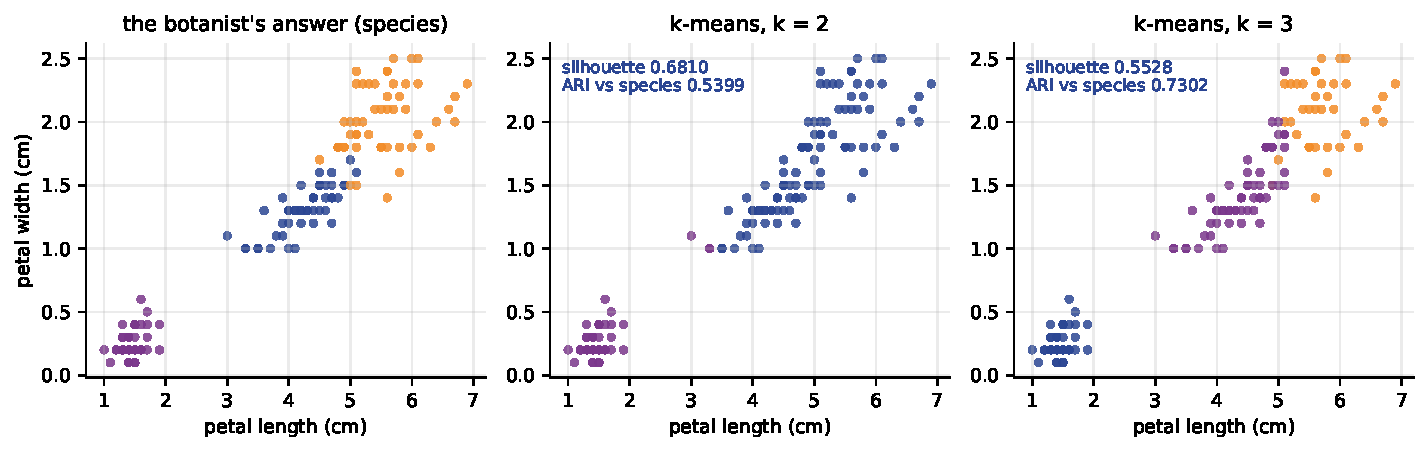
\includegraphics[width=0.99\textwidth]{twoanswers.pdf}
  \end{center}
  \begin{center}\small
    Left: what a botanist calls the truth. Middle: what the geometry calls
    the truth. \emph{Setosa} sits far away from the other two, and
    \emph{versicolor} and \emph{virginica} touch --- so a measure that
    rewards separation merges them and a measure that knows the species does
    not.
  \end{center}
\end{frame}

\begin{frame}[fragile,shrink=10]{Where the disagreement lives}
\begin{lstlisting}
two   = KMeans(n_clusters=2, n_init=10, random_state=0).fit_predict(X)
three = KMeans(n_clusters=3, n_init=10, random_state=0).fit_predict(X)
\end{lstlisting}
\begin{outblk}
                    k = 2      k = 3
silhouette         0.6810     0.5528
Calinski-Har.      513.92     561.63
Davies-Bould.      0.4043     0.6620
ARI vs labels      0.5399     0.7302
agreement between the two clusterings: ARI 0.5516
\end{outblk}
\begin{outblk}
k = 2                         k = 3
   setosa         50    0        setosa          0   50    0
   versicolor      3   47        versicolor     48    0    2
   virginica       0   50        virginica      14    0   36
\end{outblk}
  \begin{center}\small
    At $k = 2$ the second cluster is \emph{versicolor} and \emph{virginica}
    stuck together. At $k = 3$ they are split, but imperfectly: $14$
    virginica land with the versicolor. \textbf{Three internal indices, and
    they do not agree with each other either.}
  \end{center}
\end{frame}

\begin{frame}[fragile,shrink=9]{The same thing again: scaling changes the answer}
  A second, sharper version. \texttt{load\_wine}, three known cultivars,
  k-means with $k = 3$ --- run once on the raw table and once after
  standardising every column.
\begin{lstlisting}
raw = KMeans(n_clusters=3, n_init=10, random_state=0).fit_predict(Xw)
std = KMeans(n_clusters=3, n_init=10, random_state=0).fit_predict(
          StandardScaler().fit_transform(Xw))
\end{lstlisting}
\begin{outblk}
unscaled: silhouette in its own space 0.5711, ARI vs cultivar 0.3711
scaled  : silhouette in its own space 0.2849, ARI vs cultivar 0.8975
agreement between the two clusterings: ARI 0.3543
\end{outblk}
  \begin{center}\small
    Two clusterings of the same $178$ bottles that agree at ARI
    $\mathbf{0.3543}$ --- barely more than half. \textbf{Standardising is not
    a preprocessing detail here; it is the definition of ``similar''.}
  \end{center}
\end{frame}

\begin{frame}[fragile,shrink=6]{Why: one column owns the distance budget}
\begin{outblk}
share of the raw total variance held by each column
   proline                    98609.60  (99.77%)
   magnesium                    202.84  ( 0.21%)
   alcalinity_of_ash             11.09  ( 0.01%)
   color_intensity                5.34  ( 0.01%)
\end{outblk}
  \begin{columns}[T]
    \begin{column}{0.50\textwidth}
      \begin{block}{Read it}
        \texttt{proline} is measured in the hundreds; \texttt{alcohol} runs
        from $11$ to $15$. Euclidean distance on the raw table is
        \textbf{$99.77\%$ a comparison of proline}, and the other twelve
        chemical measurements are decoration.
      \end{block}
    \end{column}
    \begin{column}{0.47\textwidth}
      \begin{alertblock}{The lesson, stated once}
        Clustering has \textbf{no target to overrule your feature scaling}.
        In a supervised model a badly scaled column costs you accuracy that
        the test set reports. Here it silently redefines the question and
        nothing complains.
      \end{alertblock}
    \end{column}
  \end{columns}
\end{frame}

\begin{frame}{Drawn: the same bottles, two defensible groupings}
  \begin{center}
    
\includegraphics[width=0.99\textwidth]{scaling.pdf}
  \end{center}
  \begin{center}\small
    ``\emph{Clustering is in the eye of the beholder}'' --- Estivill-Castro,
    2002. Clustering is \textbf{exploratory}: it proposes a structure, it
    does not discover a fact. Your job is to say what you assumed, and then
    to say whether the structure is useful.
  \end{center}
\end{frame}

% =====================================================================
\section[Taxonomy]{The taxonomy of clustering algorithms}
\label{sec:tax}

\begin{frame}[shrink=13]{Five families, and what each one believes}
  \begin{center}
    \small
    \begin{tabular}{@{}lp{4.6cm}p{4.4cm}@{}}
      \toprule
      \textbf{Family} & \textbf{How it works} & \textbf{What it assumes} \\
      \midrule
      \textbf{Partitioning} & choose $k$ centres, assign each point to the
        nearest, move the centres, repeat &
        clusters are \textbf{convex blobs of similar size}, one centre each \\
      \textbf{Hierarchical} & merge the two closest clusters repeatedly
        (agglomerative) or split repeatedly (divisive) &
        depends entirely on the \textbf{linkage}: Ward assumes blobs,
        single linkage assumes connected chains \\
      \textbf{Density-based} & grow a cluster through any region whose local
        point density exceeds a threshold &
        clusters are \textbf{dense regions separated by sparse ones}; shape
        is free; density is roughly uniform \\
      \textbf{Grid-based} & lay a grid over the space, keep the dense cells,
        connect the neighbours &
        as above, plus that a \textbf{fixed resolution} is adequate \\
      \textbf{Model-based} & assume the data came from a mixture of
        distributions; fit it by maximum likelihood &
        the assumed family is right --- e.g.\ \textbf{ellipsoidal} Gaussian
        components \\
      \bottomrule
    \end{tabular}
  \end{center}
  \begin{center}\small
    Later lectures build hierarchical, partitioning and density-based
    methods in full. The point today is that \textbf{the families make
    different geometric commitments}, and those commitments are visible.
  \end{center}
\end{frame}

\begin{frame}{Predict first \#2 --- two interleaved crescents}
  \begin{alertblock}{Commit to a picture}
    Five hundred points lie on two interleaved crescent moons, each crescent
    a group. I run k-means with $k = 2$.

    \medskip
    \centering\large
    Sketch the two clusters k-means returns. Where does the boundary go?
  \end{alertblock}
  \onslide<2->{
  \begin{exampleblock}{}
    \centering\large
    A straight cut, roughly vertical. ARI $\mathbf{0.2445}$.
  \end{exampleblock}
  \begin{center}\small
    k-means assigns each point to the nearest of two centres, so its
    boundary is always the perpendicular bisector of the two centres --- a
    \textbf{straight line}. Two crescents cannot be separated by a straight
    line, so it fails, and it fails \emph{confidently}: no warning, no error,
    two clean-looking clusters. \textbf{DBSCAN gets ARI $1.0000$.}
  \end{center}}
\end{frame}

\begin{frame}{Drawn: four shapes, five algorithms, twenty answers}
  \begin{center}
    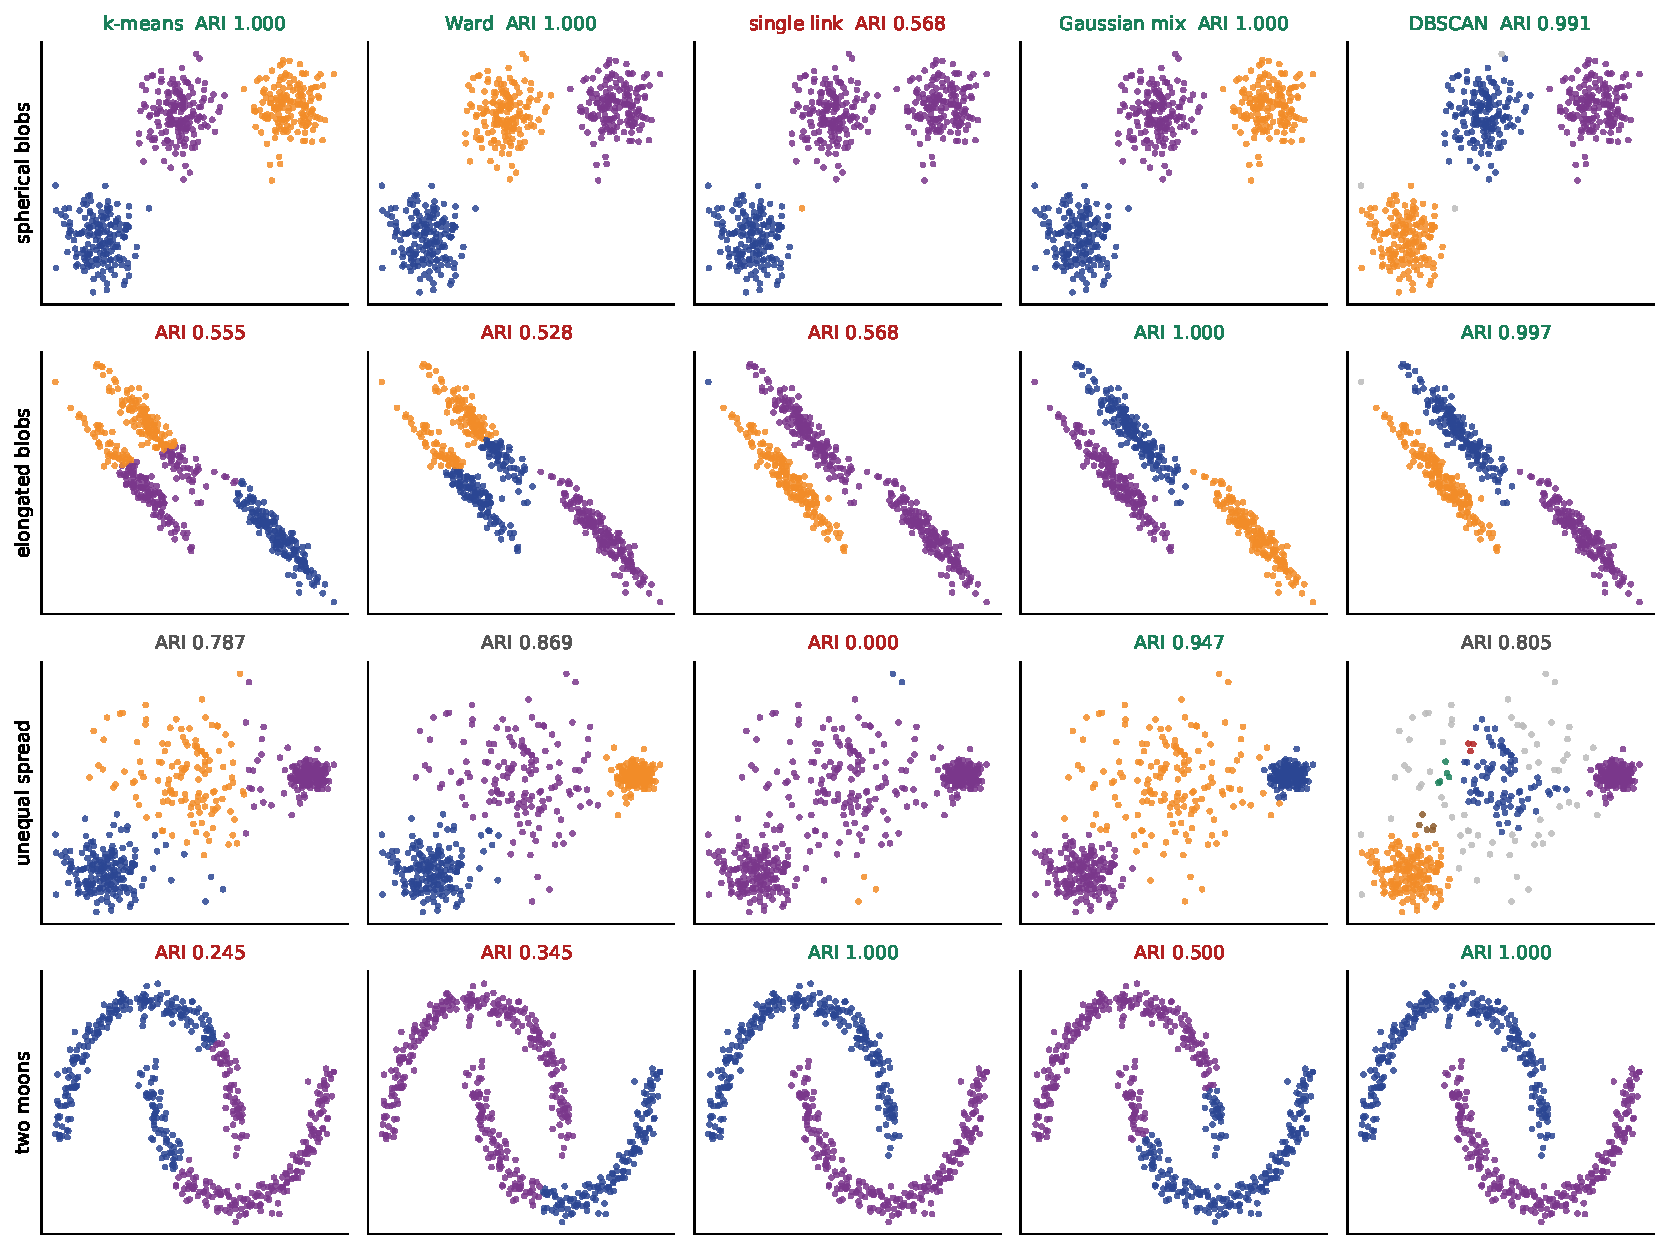
\includegraphics[height=0.74\textheight]{shapes.pdf}
  \end{center}
  \vspace{-0.4em}
  \begin{center}\footnotesize
    Green $>0.9$, red $<0.6$. \textbf{Every column has at least one red
    cell.}
  \end{center}
\end{frame}

\begin{frame}[fragile,shrink=10]{The same thing as a table}
\begin{lstlisting}
for name, X, y, eps in four_shapes():
    k = len(np.unique(y))
    print(adjusted_rand_score(y, KMeans(n_clusters=k, n_init=10,
                                        random_state=0).fit_predict(X)), ...)
\end{lstlisting}
\begin{outblk}
dataset (ARI)        KMeans      Ward    Single  GaussMix    DBSCAN
spherical blobs      1.0000    1.0000    0.5682    1.0000    0.9910
elongated blobs      0.5554    0.5281    0.5682    1.0000    0.9970
unequal spread       0.7872    0.8692    0.0002    0.9468    0.8054
two moons            0.2445    0.3447    1.0000    0.5003    1.0000
\end{outblk}
  \begin{columns}[T]
    \begin{column}{0.49\textwidth}
      \begin{block}{Read down the columns}
        k-means is perfect on round blobs and useless on moons. Single
        linkage is perfect on moons and catastrophic ($0.0002$) when the
        clusters have unequal spread --- it \emph{chains} through the sparse
        one.
      \end{block}
    \end{column}
    \begin{column}{0.49\textwidth}
      \begin{alertblock}{Read across the rows}
        \textbf{No algorithm wins every row and none is a default.} You are
        choosing a shape assumption. Pick the family whose assumption you
        believe, and then check whether the picture agrees.
      \end{alertblock}
    \end{column}
  \end{columns}
\end{frame}

\begin{frame}[fragile,shrink=10]{Grid-based, built by hand in three steps}
  Lay a $10 \times 10$ grid over the moons. Count the points in each cell.
  Keep the cells with at least $\tau = 3$. Connect the survivors.
\begin{outblk}
cell counts, x across, y up (a dot = fewer than tau = 3)
      .   .  13  21  10   .   .   .   .   .
      .  17   8   6  20  12   .   .   .   .
      4  11   .   .   .  17   3   .   .   .
     17   3   .   7   .   5  11   .   .   6
     14   .   .  12   .   .  11   .   .  15
     12   .   .  16   .   .  16   .   .  11
      9   .   .  10   6   .   6   .   .  19
      .   .   .   4  16   .   .   .  16   4
      .   .   .   .  14  19   6  17  14   .
      .   .   .   .   .   5  19   9   .   .
connected dense regions: 2
\end{outblk}
  \begin{center}\small
    Forty-three dense cells of one hundred, falling into
    \textbf{two} connected regions. ARI $\mathbf{0.9643}$, nine points left
    as noise --- and the whole algorithm is a histogram and a flood fill.
  \end{center}
\end{frame}

\begin{frame}[fragile,shrink=6]{Drawn --- and the price of the grid}
  \begin{center}
    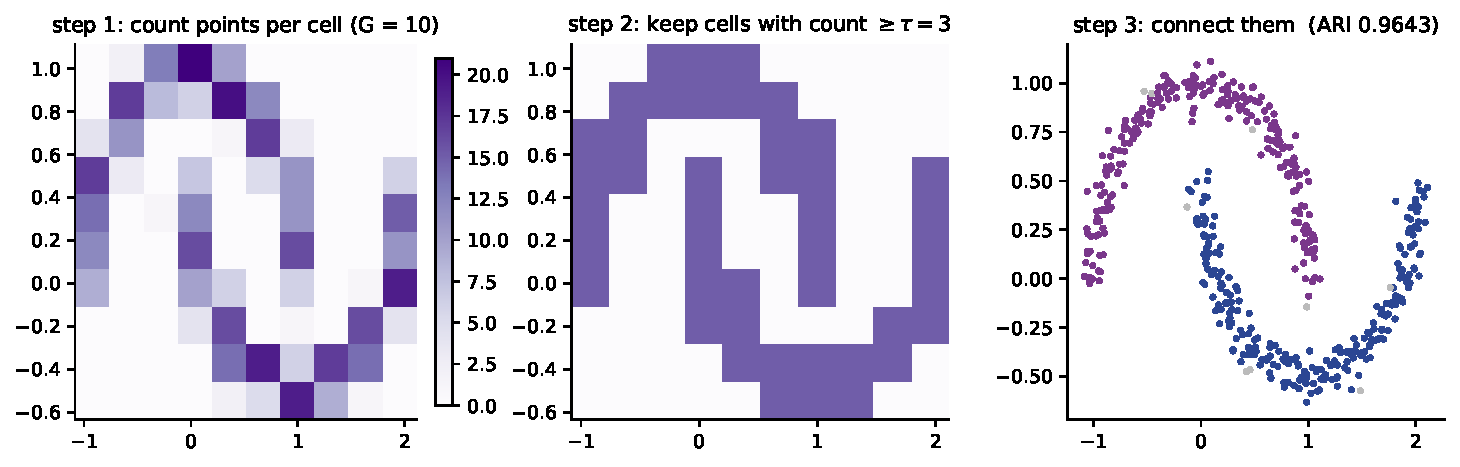
\includegraphics[width=0.82\textwidth]{gridclust.pdf}
  \end{center}
  \vspace{-0.2em}
\begin{outblk}
G=10 tau=3  dense cells  43/100  clusters 2  noise  9  ARI 0.9643
G=12 tau=2  dense cells  56/144  clusters 1  noise  9  ARI 0.0000
\end{outblk}
  \begin{center}\small
    Loosen $\tau$ by one and the two arms \textbf{bridge into a single
    cluster}: ARI collapses from $0.9643$ to $\mathbf{0.0000}$. Grid methods
    are fast --- one pass over the data, cost driven by the number of cells,
    not the number of points --- and \textbf{brittle at the resolution}.
  \end{center}
\end{frame}

% =====================================================================
\section[Statistics]{The statistics of cluster analysis}
\label{sec:stats}

\begin{frame}[shrink=6]{Three quantities, and one identity that ties them}
  Let $\bar{x}$ be the grand mean of all $n$ points and $c_j$ the
  \textbf{centroid} of cluster $j$, $c_j = \frac{1}{n_j}\sum_{x \in C_j} x$.
  \begin{columns}[T]
    \begin{column}{0.32\textwidth}
      \begin{block}{Total scatter}
        \[ T = \sum_{i=1}^{n} \lVert x_i - \bar{x}\rVert^2 \]
        A property of the \emph{data}. No clustering appears in it.
      \end{block}
    \end{column}
    \begin{column}{0.32\textwidth}
      \begin{block}{Within (WCSS)}
        \[ W = \sum_{j=1}^{k}\sum_{x \in C_j} \lVert x - c_j\rVert^2 \]
        How tight the clusters are. \emph{Smaller is better.}
      \end{block}
    \end{column}
    \begin{column}{0.32\textwidth}
      \begin{block}{Between (BCSS)}
        \[ B = \sum_{j=1}^{k} n_j \lVert c_j - \bar{x}\rVert^2 \]
        How far apart they sit. \emph{Larger is better.}
      \end{block}
    \end{column}
  \end{columns}
  \vspace{0.3em}
  \begin{exampleblock}{}
    \centering\large
    $T = W + B$ \quad --- and $T$ does not depend on the clustering.
  \end{exampleblock}
  \begin{center}\small
    So \textbf{minimising $W$ and maximising $B$ are the same problem}. That
    single sentence is why k-means only ever mentions $W$.
  \end{center}
\end{frame}

\begin{frame}[shrink=4]{By hand: six points, two clusterings}
  $P_1(2,2)$, $P_2(4,2)$, $P_3(3,5)$, $P_4(9,3)$, $P_5(11,3)$, $P_6(10,6)$.
  Grand mean $\bar{x} = (6.5,\, 3.5)$.
  \begin{columns}[T]
    \begin{column}{0.49\textwidth}
      \begin{block}{Clustering A --- left three / right three}
        \[ c_1 = \Bigl(\tfrac{2+4+3}{3}, \tfrac{2+2+5}{3}\Bigr) = (3,\,3) \]
        \[ c_2 = \Bigl(\tfrac{9+11+10}{3}, \tfrac{3+3+6}{3}\Bigr) = (10,\,4) \]
      \end{block}
    \end{column}
    \begin{column}{0.49\textwidth}
      \begin{block}{Clustering B --- low $y$ / high $y$}
        \[ c_1 = \Bigl(\tfrac{2+4+9+11}{4}, \tfrac{2+2+3+3}{4}\Bigr)
             = (6.5,\,2.5) \]
        \[ c_2 = \Bigl(\tfrac{3+10}{2}, \tfrac{5+6}{2}\Bigr) = (6.5,\,5.5) \]
      \end{block}
    \end{column}
  \end{columns}
  \begin{center}\small
    Both are legitimate partitions into two non-empty groups. A student who
    only ever sees the ``obvious'' clustering never learns what the
    statistics are \emph{for}: they are how you tell these two apart.
  \end{center}
\end{frame}

\begin{frame}[shrink=8]{By hand: $W$, $B$ and $T$ for clustering A}
  \begin{columns}[T]
    \begin{column}{0.49\textwidth}
      \begin{block}{Within, cluster by cluster}
        Cluster 1 about $(3,3)$:
        \[ (-1,-1)\!:2 \ \ (1,-1)\!:2 \ \ (0,2)\!:4 \ \Rightarrow\ 8 \]
        Cluster 2 about $(10,4)$:
        \[ (-1,-1)\!:2 \ \ (1,-1)\!:2 \ \ (0,2)\!:4 \ \Rightarrow\ 8 \]
        \[ W = 8 + 8 = \mathbf{16} \]
      \end{block}
    \end{column}
    \begin{column}{0.49\textwidth}
      \begin{block}{Between, centroid by centroid}
        \[ \lVert (3,3)-(6.5,3.5)\rVert^2 = 12.25 + 0.25 = 12.5 \]
        \[ \lVert (10,4)-(6.5,3.5)\rVert^2 = 12.25 + 0.25 = 12.5 \]
        \[ B = 3(12.5) + 3(12.5) = \mathbf{75} \]
      \end{block}
    \end{column}
  \end{columns}
  \vspace{0.2em}
  \begin{exampleblock}{}
    \centering
    Total, computed independently:
    $T = 22.5 + 8.5 + 14.5 + 6.5 + 20.5 + 18.5 = \mathbf{91}$,
    \quad and $16 + 75 = 91$. \checkmark
  \end{exampleblock}
\end{frame}

\begin{frame}[fragile,shrink=6]{The same thing in code --- and for clustering B}
\begin{lstlisting}
def scatter_decomposition(X, labels):
    g = X.mean(axis=0)
    total = ((X - g) ** 2).sum()
    within = between = 0.0
    for c in np.unique(labels):
        M = X[labels == c]; ck = M.mean(axis=0)
        within  += ((M - ck) ** 2).sum()
        between += len(M) * ((ck - g) ** 2).sum()
    return total, within, between
\end{lstlisting}
\begin{outblk}
clustering              T        W        B        W+B
A: left/right       91.00    16.00    75.00      91.00
B: low/high y       91.00    79.00    12.00      91.00
T does not depend on the clustering; W and B trade off inside it
\end{outblk}
  \begin{center}\small
    \textbf{Same $T$. Completely different split.} A is tight and far apart
    ($16 \mid 75$); B is loose and overlapping ($79 \mid 12$). The
    decomposition is the instrument that says so.
  \end{center}
\end{frame}

\begin{frame}{Drawn: the same total, split two ways}
  \begin{center}
    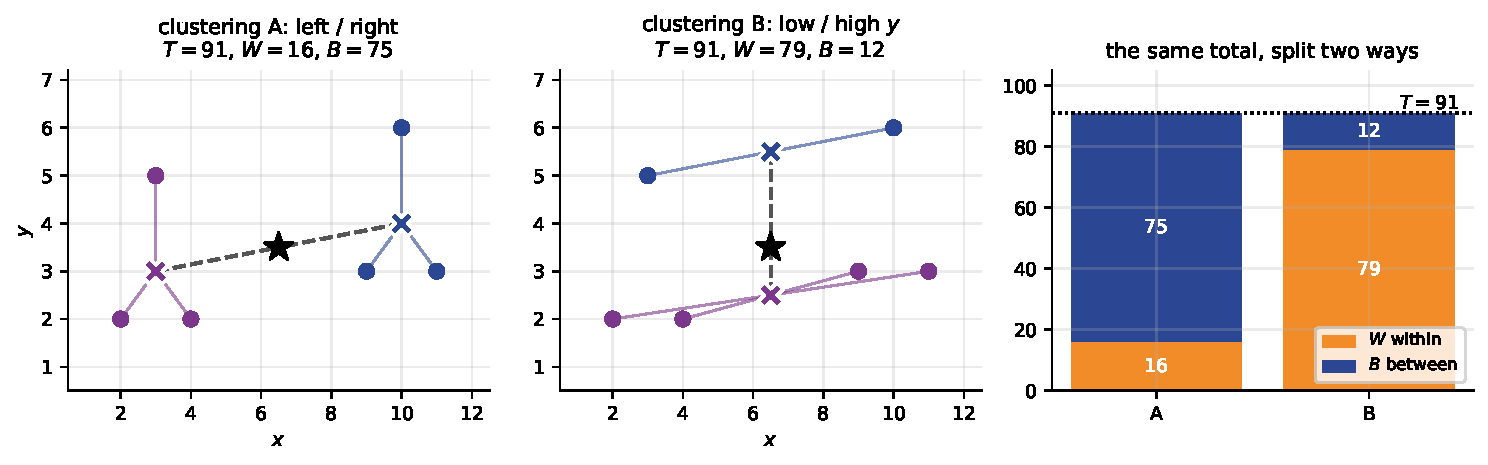
\includegraphics[width=0.95\textwidth]{decomp.pdf}
  \end{center}
  \begin{center}\small
    Coloured lines are the within-cluster distances that make $W$; dashed
    grey lines run from each centroid to the grand mean (the star) and make
    $B$. The bar on the right is the whole argument: \textbf{a fixed budget
    of $91$, and clustering is how you divide it.}
  \end{center}
\end{frame}

\begin{frame}[fragile,shrink=8]{Verified on real data, at every $k$}
\begin{lstlisting}
for k in range(1, 9):
    km = KMeans(n_clusters=k, n_init=10, random_state=0).fit(X)
    T, W, B = scatter_decomposition(X, km.labels_)
    print(k, T, W, B, abs(T - W - B))
\end{lstlisting}
\begin{outblk}
  k              T              W              B      |T-W-B|
  1     681.370600     681.370600       0.000000    0.000e+00
  2     681.370600     152.347952     529.022648    1.137e-13
  3     681.370600      78.851441     602.519159    0.000e+00
  4     681.370600      57.228473     624.142127    1.137e-13
  8     681.370600      30.064593     651.306007    0.000e+00
\end{outblk}
  \begin{center}\small
    $T = 681.370600$ at every $k$, and the residual never exceeds
    $1.14 \times 10^{-13}$ --- floating point, not mathematics. At $k = 1$
    everything is within; as $k$ grows the budget migrates into $B$.
  \end{center}
\end{frame}

\begin{frame}{Predict first \#3 --- can $W$ choose $k$?}
  \begin{alertblock}{Commit to an answer}
    $W$ measures how tight the clusters are, and smaller is better. So here
    is the obvious procedure: try every $k$, compute $W$, keep the $k$ with
    the smallest $W$.

    \medskip
    \centering\large
    What $k$ does that procedure return, on any dataset?
  \end{alertblock}
  \onslide<2->{
  \begin{exampleblock}{}
    \centering\large
    $k = n$. One point per cluster, and $W = 0$.
  \end{exampleblock}
  \begin{center}\small
    $W$ is \textbf{monotone decreasing in $k$} --- splitting a cluster can
    never increase it --- so ``minimise $W$'' is not an objective, it is a
    countdown. On iris: $681.37,\ 152.35,\ 78.85,\ 57.23,\ 46.45, \dots$
    all the way to zero. \textbf{Any method that chooses $k$ must penalise
    $k$ somehow.}
  \end{center}}
\end{frame}

\begin{frame}[shrink=4]{Drawn: monotone down, monotone up, no optimum}
  \begin{center}
    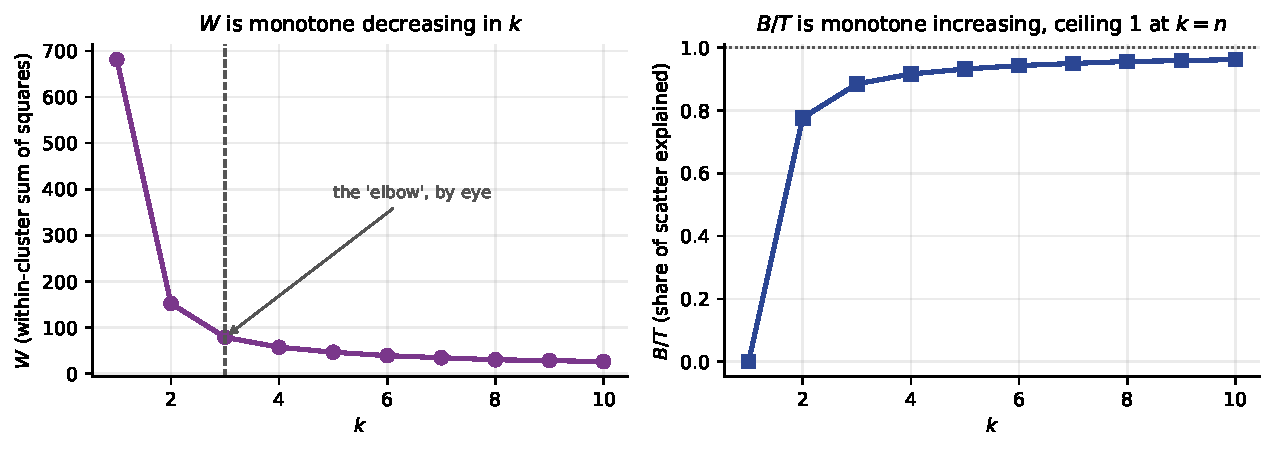
\includegraphics[width=0.90\textwidth]{elbow.pdf}
  \end{center}
  \begin{center}\small
    The ``elbow'' is a \emph{visual} heuristic on a curve with no
    mathematical optimum, and different people read a different elbow off
    the same plot. It is a starting point for a conversation, not a
    criterion. Treat it accordingly.
  \end{center}
\end{frame}

\begin{frame}[fragile,shrink=8]{Calinski--Harabasz: the decomposition, penalised}
  \begin{exampleblock}{}
    \centering\large
    $\displaystyle \mathrm{CH} = \frac{B / (k-1)}{W / (n-k)}$
    \quad --- between per degree of freedom, over within per degree of freedom.
  \end{exampleblock}
  \vspace{0.2em}
  By hand on the six points, clustering A: $B = 75$, $W = 16$, $k = 2$,
  $n = 6$, so $\mathrm{CH} = (75/1)/(16/4) = 75/4 = \mathbf{18.75}$.
  Clustering B gives $(12/1)/(79/4) = \mathbf{0.6076}$.
\begin{outblk}
A: left/right     B/T = 0.8242   CH by hand =  18.7500   sklearn =  18.7500
B: low/high y     B/T = 0.1319   CH by hand =   0.6076   sklearn =   0.6076
k=3  B/(k-1) = 301.259579   W/(n-k) =   0.536404   ratio =  561.6278
     sklearn calinski_harabasz_score = 561.6278
\end{outblk}
  \begin{center}\small
    Dividing $B$ by $k - 1$ is what stops $k = n$ from winning: adding
    clusters buys you less $B$ than it costs you in degrees of freedom. This
    index is nothing but the decomposition you just computed by hand.
  \end{center}
\end{frame}

% =====================================================================
\section[Validation]{Internal and external validation}
\label{sec:valid}

\begin{frame}[shrink=6]{Two kinds of validation, and only one is available}
  \begin{columns}[T]
    \begin{column}{0.49\textwidth}
      \begin{block}{Internal --- geometry only}
        Computed from the points and the cluster assignments. \textbf{No
        labels anywhere.} This is what you actually have.
        \begin{itemize}
          \item \textbf{Silhouette} $\in [-1,1]$, higher better
          \item \textbf{Calinski--Harabasz}, higher better
          \item \textbf{Davies--Bouldin} $\geq 0$, \emph{lower} better
        \end{itemize}
      \end{block}
    \end{column}
    \begin{column}{0.49\textwidth}
      \begin{alertblock}{External --- against known groups}
        Requires a label column you did not use for fitting. Available on
        \texttt{load\_iris} only because it happens to ship with one.
        \begin{itemize}
          \item \textbf{Adjusted Rand index} $\leq 1$, $0$ at chance
          \item \textbf{Normalised mutual information} $\in [0,1]$
        \end{itemize}
      \end{alertblock}
    \end{column}
  \end{columns}
  \begin{center}\small
    In a real clustering problem you get the left column and nothing else.
    We use iris precisely so that we can \textbf{check the left column
    against the right one} --- and find out where it is wrong.
  \end{center}
\end{frame}

\begin{frame}[shrink=6]{By hand: the silhouette of one point}
  For point $i$ in cluster $C_j$:
  \[
    a(i) = \frac{1}{n_j - 1}\!\!\sum_{x \in C_j, x \neq i}\!\! d(i,x),
    \qquad
    b(i) = \min_{l \neq j} \frac{1}{n_l}\sum_{x \in C_l} d(i,x),
    \qquad
    s(i) = \frac{b(i) - a(i)}{\max\{a(i), b(i)\}}.
  \]
  \begin{columns}[T]
    \begin{column}{0.53\textwidth}
      \begin{block}{$P_1(2,2)$ in clustering A}
        $a$: distances to $P_2$ and $P_3$ are $2$ and
        $\sqrt{10} = 3.162278$, so
        $a = 5.162278/2 = 2.581139$.\\[0.3em]
        $b$: to $P_4, P_5, P_6$ they are $\sqrt{50}=7.071068$,
        $\sqrt{82}=9.055385$, $\sqrt{80}=8.944272$, so $b = 8.356908$.\\[0.3em]
        $s = (8.356908 - 2.581139)/8.356908 = \mathbf{0.691137}$.
      \end{block}
    \end{column}
    \begin{column}{0.45\textwidth}
      \begin{alertblock}{What the three numbers mean}
        $a$ is ``how far am I from my own people''. $b$ is ``how far from the
        nearest other crowd''. $s$ near $\mathbf{+1}$: comfortably placed.
        Near $\mathbf{0}$: on the border. \textbf{Negative: closer to another
        cluster than to your own} --- probably misassigned.
      \end{alertblock}
    \end{column}
  \end{columns}
\end{frame}

\begin{frame}[fragile,shrink=10]{All six, and the library agrees exactly}
\begin{lstlisting}
D = cdist(P6, P6)
s = silhouette_samples(P6, LAB_A)
\end{lstlisting}
\begin{outblk}
point       a(i)      b(i)      s(i)   sklearn
  P1    2.581139  8.356908  0.691137  0.691137
  P2    2.581139  6.460397  0.600467  0.600467
  P3    3.162278  7.213945  0.561644  0.561644
  P4    2.581139  6.164881  0.581316  0.581316
  P5    2.581139  8.124221  0.682291  0.682291
  P6    3.162278  7.742147  0.591550  0.591550
mean silhouette  0.618068   sklearn 0.618068
clustering B     -0.071164   sklearn -0.071164
\end{outblk}
  \begin{center}\small
    Clustering B scores $\mathbf{-0.071164}$ --- negative, meaning the
    average point is nearer the \emph{other} cluster's members than its own.
    The silhouette does not merely prefer A; it says B is actively wrong.
  \end{center}
\end{frame}

\begin{frame}[fragile,shrink=8]{Davies--Bouldin, in one line}
  \[
    \mathrm{DB} = \frac{1}{k}\sum_{j=1}^{k}\ \max_{l \neq j}
    \frac{S_j + S_l}{d(c_j, c_l)},
    \qquad
    S_j = \frac{1}{n_j}\sum_{x \in C_j} \lVert x - c_j \rVert .
  \]
  For every cluster, find its \emph{worst} neighbour --- the one whose
  combined spread is largest relative to the centroid distance --- and
  average those worst cases. \textbf{Lower is better}, and $0$ is
  unattainable.
  \begin{columns}[T]
    \begin{column}{0.49\textwidth}
      \begin{block}{Three indices, three formulas}
        Silhouette works on \textbf{pairwise distances}; CH works on the
        \textbf{scatter decomposition}; DB works on \textbf{centroid
        spreads}. They measure related but different things.
      \end{block}
    \end{column}
    \begin{column}{0.49\textwidth}
      \begin{alertblock}{So expect them to disagree}
        And they do, on the very next slide. An index is a summary of a
        partition into one number; three different summaries of the same
        partition need not rank two partitions the same way.
      \end{alertblock}
    \end{column}
  \end{columns}
\end{frame}

\begin{frame}[fragile,shrink=9]{All three across $k$, no labels used}
\begin{lstlisting}
for k in range(2, 9):
    lab = KMeans(n_clusters=k, n_init=10, random_state=0).fit_predict(X)
    print(k, silhouette_score(X, lab), calinski_harabasz_score(X, lab),
             davies_bouldin_score(X, lab))
\end{lstlisting}
\begin{outblk}
  k   silhouette           CH           DB |        ARI        NMI
  2       0.6810       513.92       0.4043 |     0.5399     0.6565
  3       0.5528       561.63       0.6620 |     0.7302     0.7582
  4       0.4981       530.77       0.7803 |     0.6498     0.7219
  5       0.4887       495.54       0.8060 |     0.6079     0.6939
  6       0.3648       473.85       0.9142 |     0.4475     0.6380
  7       0.3569       447.96       0.9628 |     0.4813     0.6689
  8       0.3597       439.46       0.9266 |     0.4570     0.6581
\end{outblk}
  \begin{center}\small
    Silhouette picks $k=2$. Calinski--Harabasz picks $k=3$. Davies--Bouldin
    picks $k=2$. \textbf{Two of the three internal indices disagree with the
    species}, which pick $k=3$ by both external measures.
  \end{center}
\end{frame}

\begin{frame}{Drawn: the internal indices, and where each one peaks}
  \begin{center}
    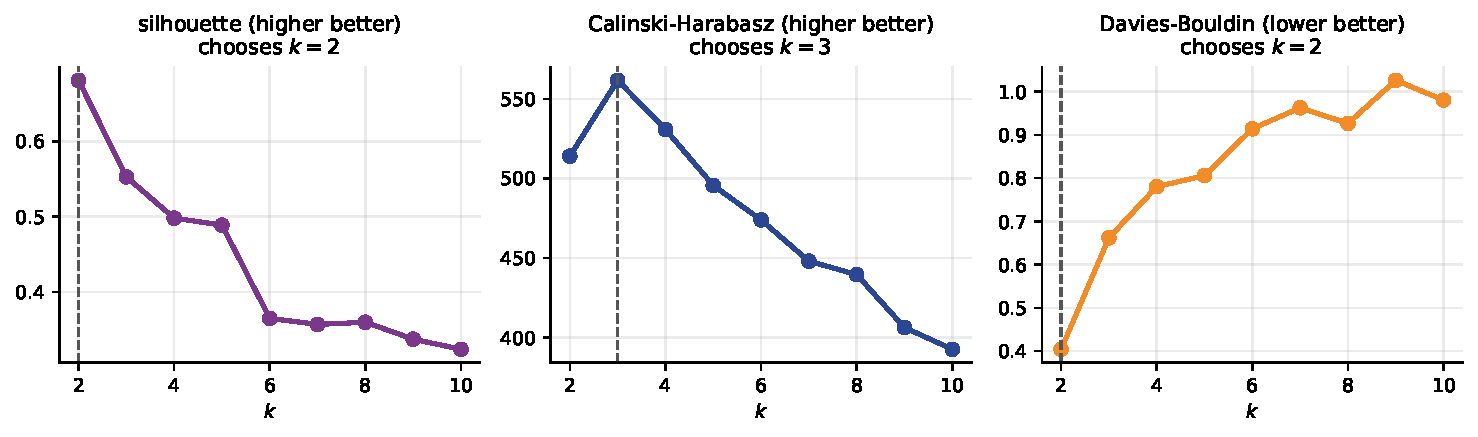
\includegraphics[width=0.99\textwidth]{internal.pdf}
  \end{center}
  \begin{center}\small
    Report the ones that disagree with you. A single index quoted alone is a
    number chosen after the fact to support a decision already taken.
  \end{center}
\end{frame}

\begin{frame}[shrink=3]{Drawn: unsupervised score against ground truth}
  \begin{columns}[T]
    \begin{column}{0.56\textwidth}
      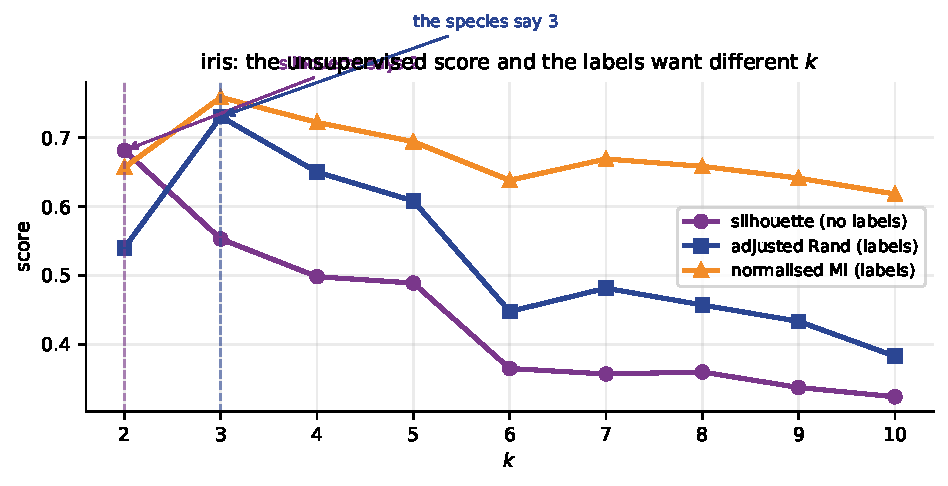
\includegraphics[width=\textwidth]{external.pdf}
    \end{column}
    \begin{column}{0.42\textwidth}
      \begin{alertblock}{Be honest about this}
        The silhouette \textbf{prefers a clustering the labels do not}.
        $k = 2$ scores $0.6810$ but merges two of the three species; $k = 3$
        scores only $0.5528$ and recovers them.
      \end{alertblock}
      \begin{block}{And say why}
        Silhouette rewards \emph{separation}. \emph{Versicolor} and
        \emph{virginica} genuinely overlap in these four measurements, so a
        separation-based score is right to dislike the boundary between
        them. It is answering its own question correctly. It is simply not
        answering the botanist's question.
      \end{block}
    \end{column}
  \end{columns}
\end{frame}

\begin{frame}{Predict first \#4 --- what does random labelling score?}
  \begin{alertblock}{Commit to a number}
    Take iris. Ignore the data entirely. Assign each of the $150$ flowers a
    cluster in $\{0,1,2\}$ by rolling a die. Score that against the true
    species with the plain \textbf{Rand index} --- the fraction of point
    pairs the two partitions agree about.

    \medskip
    \centering\large
    What does pure noise score?
  \end{alertblock}
  \onslide<2->{
  \begin{exampleblock}{}
    \centering\large
    $\mathbf{0.5567}$. Over half, from nothing at all.
  \end{exampleblock}
  \begin{center}\small
    The \textbf{adjusted} Rand index subtracts the expected value under
    random labelling: it scores $\mathbf{-0.0010}$. NMI scores $0.0114$.
    \textbf{Always report the adjusted form}, and treat any unadjusted
    agreement statistic near $0.5$ as evidence of nothing.
  \end{center}}
\end{frame}

\begin{frame}[fragile,shrink=8]{Cluster numbers are names, not classes}
\begin{lstlisting}
lab3 = KMeans(n_clusters=3, n_init=10, random_state=0).fit_predict(X)
perm = np.array([{0: 2, 1: 0, 2: 1}[v] for v in lab3])   # rename only
\end{lstlisting}
\begin{outblk}
   ARI before 0.730238   after 0.730238
   NMI before 0.758176   after 0.758176
200 completely random 3-way labellings of iris
   Rand index                   mean +0.5567  sd 0.0035
   adjusted Rand index          mean -0.0010  sd 0.0073
   normalised mutual info       mean +0.0114  sd 0.0067
\end{outblk}
  \begin{center}\small
    Renaming the clusters changes nothing, because ARI and NMI are functions
    of the \textbf{partition}, not of the labels. This is also why
    \texttt{accuracy\_score(y, clusters)} is meaningless: cluster $0$ is not
    class $0$, it is just the first group the algorithm happened to build.
  \end{center}
\end{frame}

\begin{frame}[shrink=2]{Drawn: the silhouette profile, which the mean hides}
  \begin{center}
    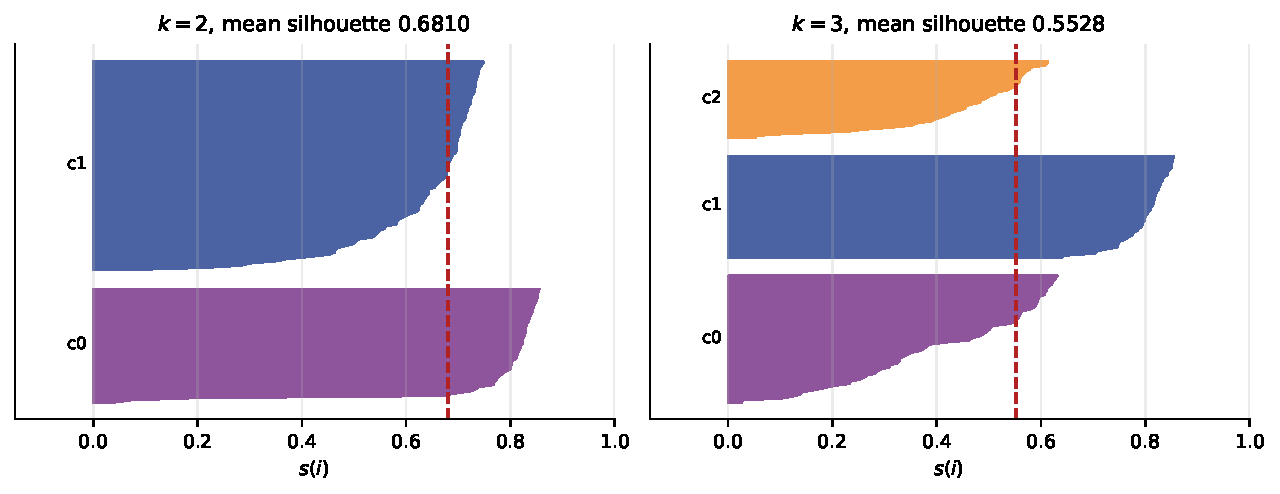
\includegraphics[width=0.86\textwidth]{silprofile.pdf}
  \end{center}
  \begin{center}\small
    At $k = 3$ the three clusters score $0.4173$, $\mathbf{0.7981}$ and
    $0.4511$: one crisp cluster (\emph{setosa}) and two mediocre ones. The
    mean of $0.5528$ conceals that entirely. \textbf{Plot the profile, not
    just the average.}
  \end{center}
\end{frame}

% =====================================================================
\section[Preprocessing]{Clustering as a preprocessing tool}
\label{sec:prep}

\begin{frame}[shrink=6]{Two ways clustering feeds a supervised model}
  \begin{columns}[T]
    \begin{column}{0.49\textwidth}
      \begin{block}{1. Cluster membership as a feature}
        Fit k-means on the training rows. Append the cluster indicator (or
        the $k$ distances to the centroids) to $X$. A \textbf{linear} model
        then gets a piecewise, non-linear view of the space for the price of
        $k$ extra columns.
      \end{block}
    \end{column}
    \begin{column}{0.49\textwidth}
      \begin{block}{2. Cluster-then-label}
        Labels cost money; rows are free. Cluster the unlabelled rows, label
        \textbf{one representative per cluster}, and either train on those
        few or propagate each label to its whole cluster. This is how a
        labelling budget should be spent.
      \end{block}
    \end{column}
  \end{columns}
  \begin{alertblock}{And the rule that governs both}
    Fit the clusterer on the \textbf{training rows only}, then
    \texttt{predict} on the test rows. Fitting k-means on all the data before
    splitting leaks the test set into the features --- the same leakage rule
    as scaling, wearing a new hat.
  \end{alertblock}
\end{frame}

\begin{frame}[fragile,shrink=10]{Measured: cluster indicators on the moons}
\begin{lstlisting}
km  = KMeans(n_clusters=k, n_init=10, random_state=0).fit(Xtr)
Otr = np.eye(k)[km.labels_];  Ote = np.eye(k)[km.predict(Xte)]
LogisticRegression(max_iter=5000).fit(np.hstack([Xtr, Otr]), ytr)
\end{lstlisting}
\begin{outblk}
logistic regression on the two raw columns   0.9056
    k      + one-hot    + distances
    2         0.9444         0.9667
    4         0.9722         0.9167
    6         0.9889         0.9778
    8         0.9944         0.9833
   10         0.9944         0.9833
   15         0.9944         0.9889
   20         0.9889         0.9889
\end{outblk}
  \begin{center}\small
    $0.9056 \to \mathbf{0.9944}$ --- a linear model that could not bend now
    bends, because the eight cluster indicators carve the plane into eight
    regions and the model fits an intercept in each. \textbf{The labels were
    never used to build those regions.}
  \end{center}
\end{frame}

\begin{frame}{Drawn: where the extra columns come from}
  \begin{center}
    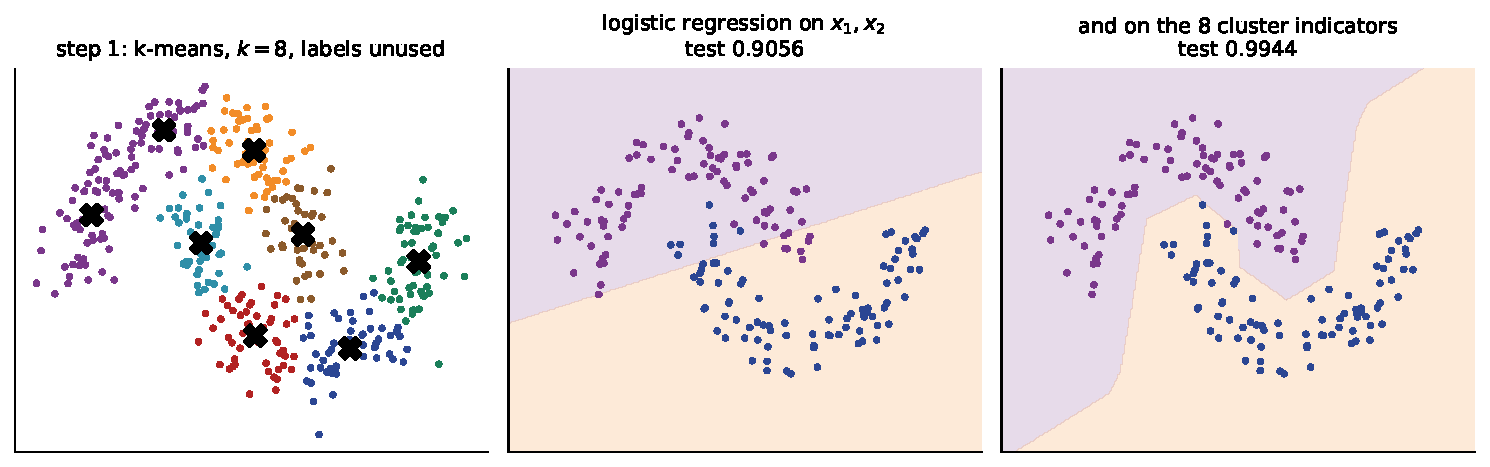
\includegraphics[width=0.99\textwidth]{features.pdf}
  \end{center}
  \begin{center}\small
    Left: k-means run on the training rows with the labels hidden. Middle:
    logistic regression on two columns can only draw a line. Right: the same
    model, plus eight indicator columns, now draws a boundary that follows
    the cluster edges.
  \end{center}
\end{frame}

\begin{frame}[fragile,shrink=6]{And the null result, reported as it happened}
\begin{outblk}
logistic regression on the 30 scaled columns  0.9591
   +  2 cluster distances                     0.9532
   +  5 cluster distances                     0.9591
   + 10 cluster distances                     0.9649
   + 20 cluster distances                     0.9591
\end{outblk}
  \begin{columns}[T]
    \begin{column}{0.49\textwidth}
      \begin{block}{On \texttt{breast\_cancer}, it buys nothing}
        Best case $+0.0058$, or \textbf{one test patient out of $171$}. Two
        of the four settings made it worse. This is not a result; it is
        noise.
      \end{block}
    \end{column}
    \begin{column}{0.49\textwidth}
      \begin{alertblock}{Why the moons and not this}
        The trick pays when the \textbf{decision boundary is non-linear and
        the clusters line up with it}. Here thirty scaled columns are already
        close to linearly separable, so there is nothing for the extra
        columns to add. \textbf{Measure it; do not assume it.}
      \end{alertblock}
    \end{column}
  \end{columns}
\end{frame}

\begin{frame}[fragile,shrink=10]{Cluster-then-label: spending fifty labels well}
\begin{lstlisting}
km  = KMeans(n_clusters=B, n_init=10, random_state=0).fit(Xtr)
rep = np.argmin(km.transform(Xtr), axis=0)   # one nearest-to-centroid row
yprop = np.empty(len(Xtr), int)
for i in range(B): yprop[km.labels_ == i] = ytr[rep[i]]
\end{lstlisting}
\begin{outblk}
fully supervised baseline (1257 labels) 0.9722
 budget     random       sd   representative    propagated
     10     0.4744   0.0180           0.7926        0.7741
     20     0.6378   0.0337           0.8463        0.9000
     30     0.7219   0.0374           0.9056        0.9111
     50     0.8104   0.0274           0.8981        0.9389
    100     0.8907   0.0184           0.9370        0.9370
\end{outblk}
  \begin{center}\small
    Fifty labels chosen \emph{by clustering}, then propagated, reach
    $\mathbf{0.9389}$ --- against $0.8104$ for fifty labels chosen at random,
    and $0.9722$ for all $1257$. \textbf{Ninety-six per cent of the
    achievable accuracy for four per cent of the labelling.}
  \end{center}
\end{frame}

\begin{frame}[fragile]{Drawn: three ways to spend the same budget}
  \begin{columns}[T]
    \begin{column}{0.56\textwidth}
      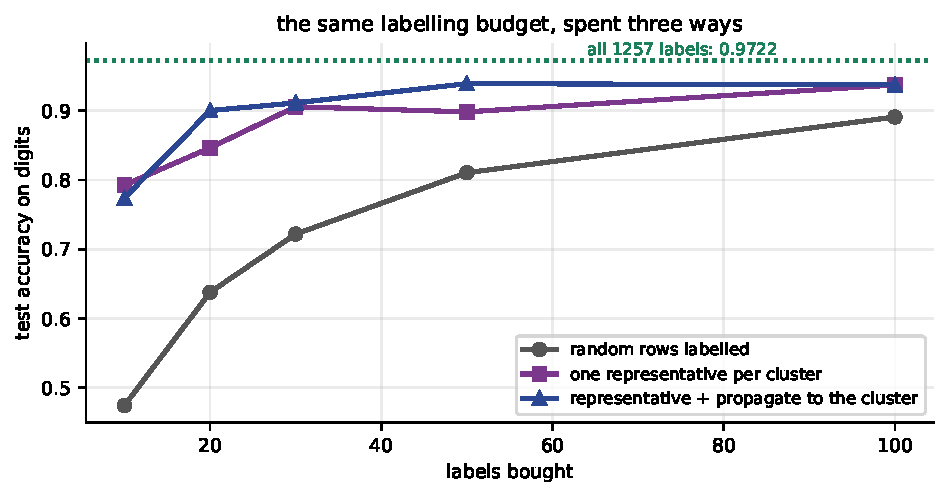
\includegraphics[width=\textwidth]{budget.pdf}
    \end{column}
    \begin{column}{0.42\textwidth}
\begin{outblk}
50 labels bought; 1257 rows
labelled by propagation
correct: 1206 of 1257 (0.9594)
trains on 4.06% wrong labels
\end{outblk}
      \begin{block}{Why propagation still wins}
        It introduces $51$ wrong labels. It also multiplies the training set
        by $25$. Logistic regression tolerates $4\%$ label noise far better
        than it tolerates having only fifty rows.
      \end{block}
    \end{column}
  \end{columns}
\end{frame}

% =====================================================================
\section[Applications]{General applications of clustering}
\label{sec:apps}

\begin{frame}[shrink=8]{Where this actually gets used}
  \begin{columns}[T]
    \begin{column}{0.49\textwidth}
      \begin{block}{Segmentation}
        \textbf{Customers} by purchase behaviour, so that a campaign can be
        written for each group rather than for an average nobody resembles.
        \textbf{Students} by attempt patterns, to decide who needs which
        intervention.
      \end{block}
      \begin{block}{Organising a corpus}
        \textbf{Documents} into topics for browsing; \textbf{search results}
        grouped so a query with two meanings returns two piles;
        \textbf{genes} with correlated expression profiles.
      \end{block}
    \end{column}
    \begin{column}{0.49\textwidth}
      \begin{block}{Compression and summarisation}
        \textbf{Vector quantisation}: replace every value by its cluster
        centre. Colour palettes, codebooks, and the first step of many
        retrieval systems.
      \end{block}
      \begin{block}{Anomaly detection}
        Points in no cluster, or in a cluster of size one, are candidates:
        \textbf{fraudulent transactions}, \textbf{intrusions}, \textbf{faulty
        sensors}. DBSCAN gives you this for free --- it already refuses to
        assign some points.
      \end{block}
    \end{column}
  \end{columns}
\end{frame}

\begin{frame}[fragile,shrink=5]{Measured: colour quantisation is clustering}
  Treat each pixel as a point in $\mathbb{R}^3$. Cluster the colours. Replace
  every pixel by its cluster centre.
\begin{outblk}
image 427 x 640 pixels, 96615 distinct colours
   k=  2  palette   2 colours  MSE 0.019764  storage  4.17% of 24-bit
   k=  4  palette   4 colours  MSE 0.007028  storage  8.34% of 24-bit
   k=  8  palette   8 colours  MSE 0.003246  storage 12.51% of 24-bit
   k= 16  palette  16 colours  MSE 0.001792  storage 16.69% of 24-bit
   k= 32  palette  32 colours  MSE 0.000998  storage 20.88% of 24-bit
\end{outblk}
  \begin{center}
    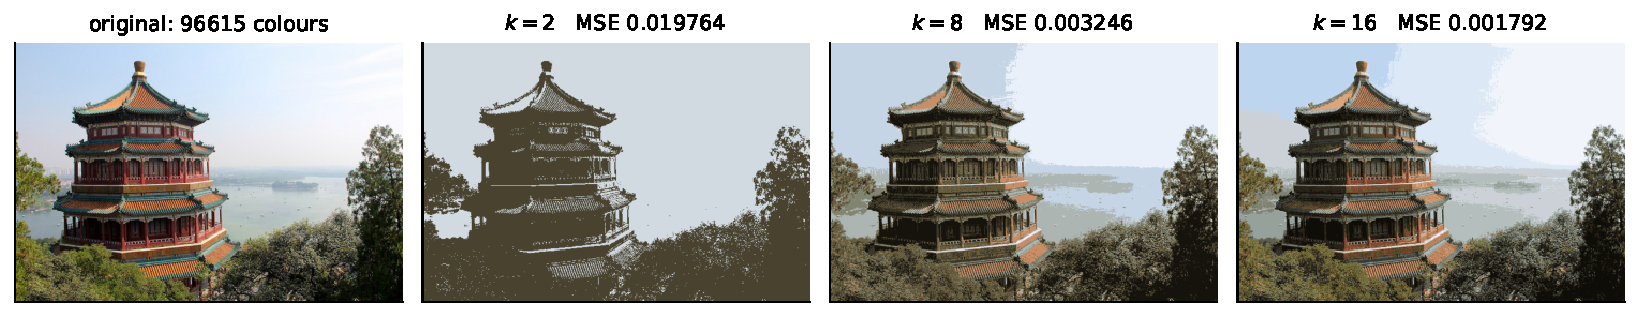
\includegraphics[width=0.86\textwidth]{quantise.pdf}
  \end{center}
\end{frame}

\begin{frame}[fragile,shrink=9]{Measured: digits, with the labels hidden}
\begin{outblk}
k-means with k=10 on 1797 unlabelled digit images
   ARI vs the true digit 0.6657, NMI 0.7425
   cluster : dominant digit (purity)
      0 : 0 (176 of 178 = 0.99)      5 : 6 (177 of 182 = 0.97)
      1 : 1 (100 of 223 = 0.45)      6 : 4 (165 of 169 = 0.98)
      2 : 7 (174 of 208 = 0.84)      7 : 5 (136 of 150 = 0.91)
      3 : 1 ( 54 of  87 = 0.62)      8 : 9 (139 of 247 = 0.56)
      4 : 3 (154 of 178 = 0.87)      9 : 2 (148 of 175 = 0.85)
   overall purity 0.7919
\end{outblk}
  \begin{center}\small
    Knowing nothing but $64$ pixel values, k-means finds groups that are
    $79\%$ pure. Zeros, sixes and fours come out almost perfectly. The
    failures are honest ones: \textbf{ones are split across two clusters},
    and nines and eights are confused --- which is roughly what a human
    confuses too.
  \end{center}
\end{frame}

% =====================================================================
\section{Summary}
\label{sec:summary}

\begin{frame}[shrink=22]{Summary --- twelve lines}
  \begin{enumerate}\small
    \item Clustering has \textbf{no target column}, so the objective is a
      modelling choice and validation must be rebuilt from geometry.
    \item \textbf{There is no single right answer.} On iris the silhouette
      prefers $k=2$ ($0.6810$ against $0.5528$) and the species prefer $k=3$
      (ARI $0.7302$ against $0.5399$). The two clusterings agree at ARI
      $\mathbf{0.5516}$.
    \item Feature scaling \emph{is} the definition of similar. On wine,
      raw against standardised gives ARI to the cultivar of $0.3711$ and
      $\mathbf{0.8975}$, and the two clusterings agree at only $0.3543$ ---
      because \texttt{proline} holds $99.77\%$ of the raw variance.
    \item Five families: \textbf{partitioning, hierarchical, density-based,
      grid-based, model-based}, each committing to a different cluster shape.
    \item Those commitments have teeth. On two moons k-means scores
      $\mathbf{0.2445}$ and DBSCAN $\mathbf{1.0000}$; on unequal spread
      single linkage scores $\mathbf{0.0002}$ and the Gaussian mixture
      $0.9468$. \textbf{No algorithm wins all four datasets.}
    \item A grid clusterer is a histogram plus a flood fill: $43$ dense
      cells of $100$, two components, ARI $0.9643$ --- and at $\tau = 2$ the
      arms bridge and it collapses to $\mathbf{0.0000}$.
    \item \textbf{$T = W + B$.} On six points: $91 = 16 + 75$ for one
      clustering and $91 = 79 + 12$ for another. On iris,
      $T = 681.370600$ at every $k$, residual $\leq 1.14\text{e}{-13}$.
    \item $T$ is fixed, so \textbf{minimising $W$ and maximising $B$ are one
      problem}. $W$ is monotone decreasing in $k$ and reaches $0$ at $k = n$,
      so it cannot choose $k$; the elbow is a heuristic, not an optimum.
    \item $\mathrm{CH} = \frac{B/(k-1)}{W/(n-k)}$ is the decomposition with
      the degrees of freedom put back: $75/4 = 18.75$ by hand, $18.7500$ from
      \texttt{scikit-learn}.
    \item Silhouette: $s(i) = (b-a)/\max(a,b)$. By hand $P_1$ gives
      $\mathbf{0.691137}$; the mean over the six is $0.618068$ and the rival
      clustering is $\mathbf{-0.071164}$ --- negative means misassigned.
    \item External measures must be \textbf{chance-corrected}: a random
      3-way labelling of iris scores Rand $\mathbf{0.5567}$ but ARI
      $\mathbf{-0.0010}$. Renaming clusters changes neither ARI nor NMI, so
      ``accuracy'' is undefined.
    \item As preprocessing it works when it works: moons
      $0.9056 \to \mathbf{0.9944}$ with eight cluster indicators;
      \texttt{breast\_cancer} $0.9591 \to 0.9649$, which is one patient.
      Cluster-then-label reaches $\mathbf{0.9389}$ on $50$ labels against
      $0.8104$ spent at random.
  \end{enumerate}
\end{frame}

\begin{frame}[shrink=3]{Before the next lecture}
  \begin{columns}[T]
    \begin{column}{0.48\textwidth}
      \begin{block}{Read}
        \texttt{notes.pdf} --- the decomposition proved, the silhouette
        derived, the taxonomy in full, and \textbf{practice questions with
        complete worked solutions}.
      \end{block}
      \begin{block}{Do}
        Take the six points, invent a \emph{third} clustering, and compute
        $W$, $B$, $T$, CH and the mean silhouette with a pen. Check that $T$
        still comes to $91$. If it does not, one of your centroids is wrong.
      \end{block}
    \end{column}
    \begin{column}{0.48\textwidth}
      \begin{exampleblock}{The habit to take away}
        Before you cluster anything, write down \textbf{what similar means}
        and \textbf{what you will do with the groups}. Both answers change
        the algorithm you should pick, and neither is in the data file.
      \end{exampleblock}
      \begin{alertblock}{And the habit to unlearn}
        Do not report one silhouette and call the clustering validated.
        Report at least two indices, plot the profile, look at the clusters,
        and say plainly which measures disagreed with you.
      \end{alertblock}
    \end{column}
  \end{columns}
  \begin{center}
    \small Next: what ``similar'' means for binary, nominal and ordinal
    columns --- the distances this lecture kept assuming.
    \quad Materials: \texttt{\AMLRepoURL}
  \end{center}
  \slidesources{\AMLUnitVIISources}
\end{frame}

\end{document}
